%!TEX root =  ../D5.4.tex

\section{Experimental Results}
%
In this Section we discuss the evaluation procedure to prove the computation effectiveness of
 our estimation algorithm. The analysis was mainly performed on Matlab. 
 %and the related code 
%is freely available on Github\footnote{\texttt{https://github.com/claudia-lat/MAPest}}.
%
%%%%%%%%%%%%%%%%%%%%%%%%%%%%%%%%%%%%%%%%%%%%%%%%%%%%%%%%%%%%%%%%%%%%%%%%%%%%%%%%%%%%%%%%%%%%%%%%
\subsection{Torques estimation}
The core of the experiment consists in estimating the
 variable $\bm d$.  Among the variables contained in $\bm d$, the quantities of major 
 interest in our analysis are 
 the torques $\bm{\tau}$. We consider the internal
 torques developed along the $y$ axis in which the most significant angle variation is observed. 
In particular, we take into account the torque at the hip for $BT$ and the knee for $ST$. Since
 the torque estimation provides qualitatively a comparable result for both the two sides of 
 the human body, it is exhaustive to show only the torques associated to one side, e.g. the
  right one.
The value of the torque mostly depends on the kinematics and further on the 
inertial parameters of the subject and therefore, in order to compare torques across different subjects,
 it has to be normalized by considering the maximum and minimum values of each 
 subject's torque. 
Figures \ref{fig:figs_torqueRightHipBH}-\ref{fig:figs_torqueRightHipBRA} show the mean 
and the standard deviation of the right hip $\bm{\tau}$ estimation  without and 
with the interaction with the robot, respectively.  Figures \ref{fig:figs_torqueRightKneeSH}-\ref{fig:figs_torqueRightKneeSR} show the same 
quantities for the torques at the right knee in a $ST$ task.
%
% \begin{figure}[h!]
%   \centering
%    \begin{subfigure}[b]{0.49\columnwidth}
%       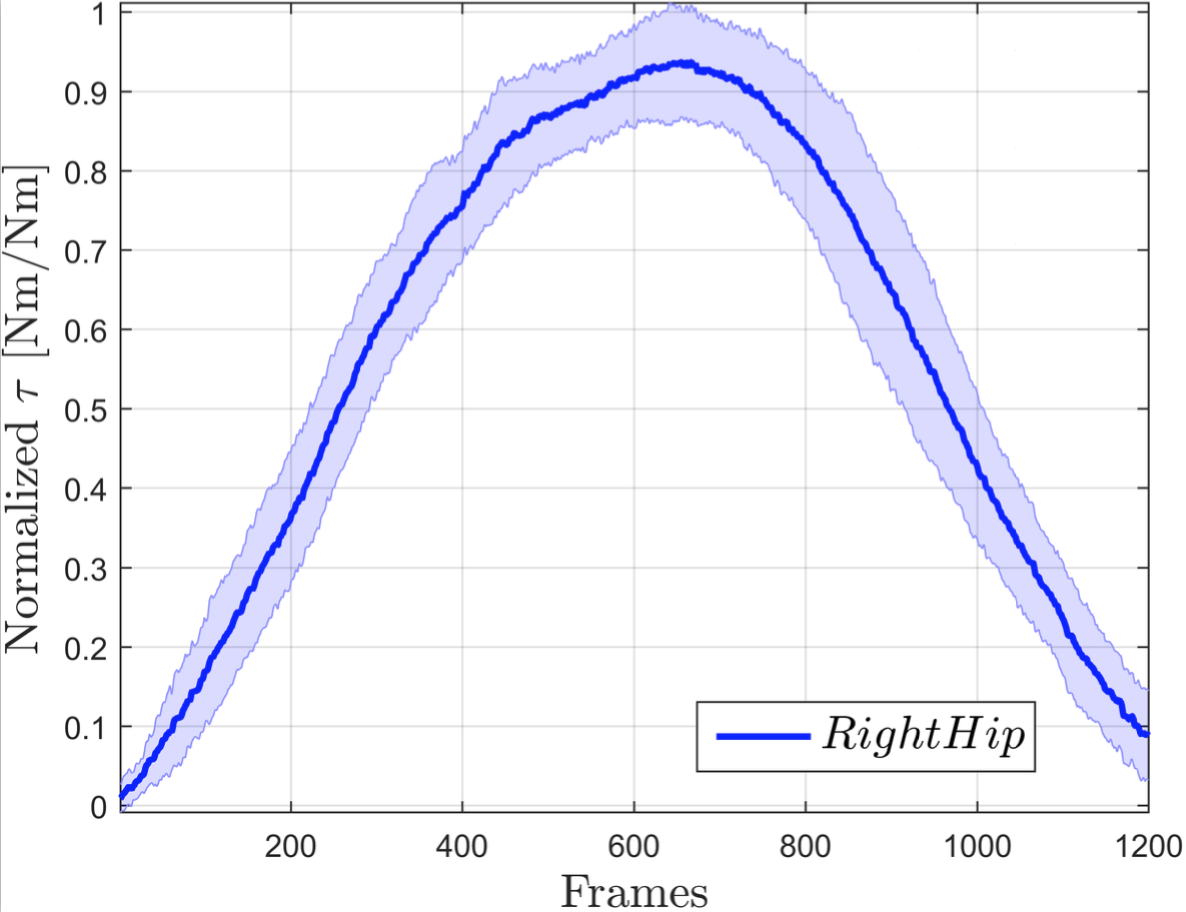
\includegraphics[width=\textwidth]{figs/torqueRightHipBH.pdf}
%           \caption{}
%           \label{fig:figs_torqueRightHipBH}
%   \end{subfigure}
%    \begin{subfigure}[b]{0.49\columnwidth}
%     \includegraphics[width=\textwidth]{figs/torqueRightHipBRA.pdf}
% 	\caption{}
%         \label{fig:figs_torqueRightHipBRA}
%    \end{subfigure}
%    \begin{subfigure}[b]{0.49\columnwidth}
%     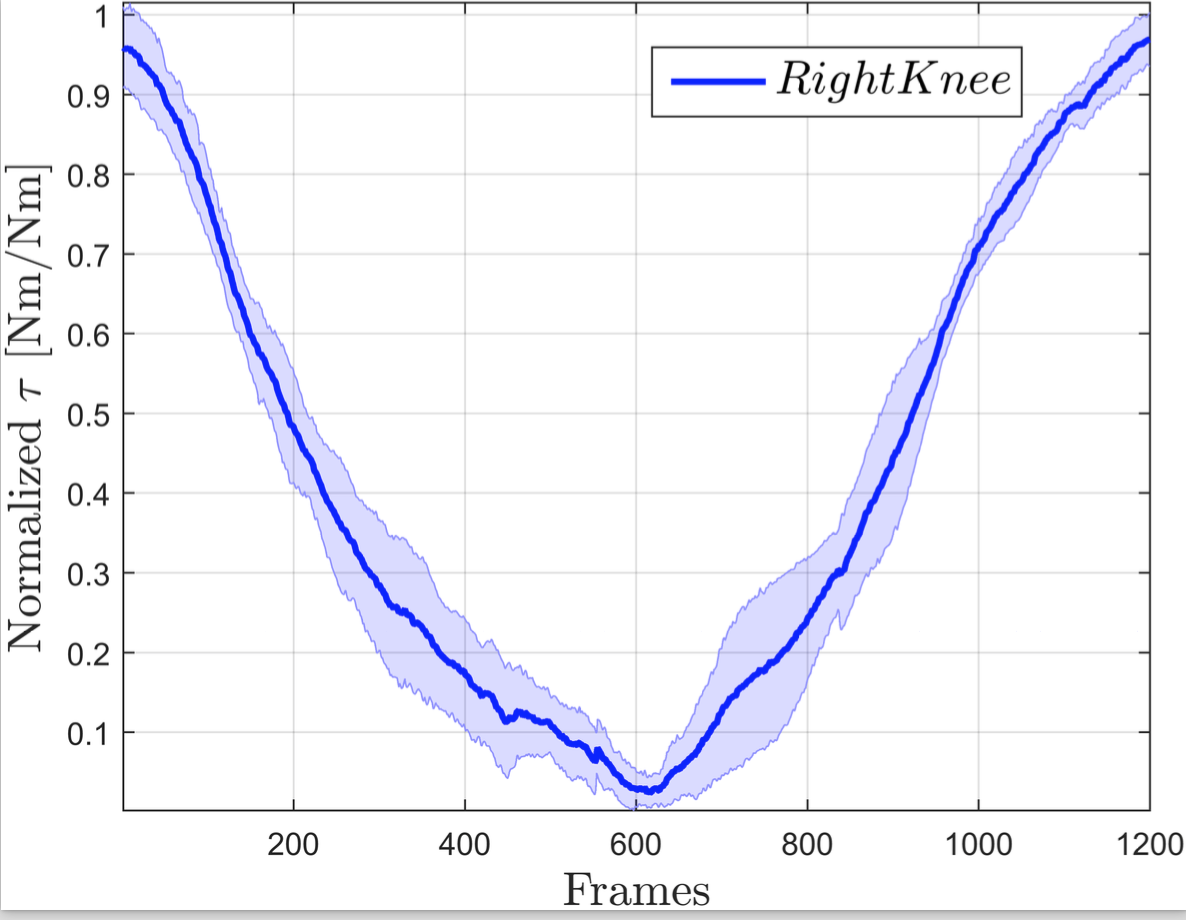
\includegraphics[width=\textwidth]{figs/torqueRightKneeSH.pdf}
% 	\caption{}
%         \label{fig:figs_torqueRightKneeSH}
%    \end{subfigure}
%    \begin{subfigure}[b]{0.49\columnwidth}
%     \includegraphics[width=\textwidth]{figs/torqueRightKneeSR.pdf}
% 	\caption{}
%         \label{fig:figs_torqueRightKneeSR}
%    \end{subfigure}
%           \caption{\emph{Inter-subjects analysis}: normalised right hip torques of 10 subjects
% 		  (mean and standard deviation) for BT without (a) and with (b) robot, for ST without
% 		   (c) and with (d) robot.}
% \end{figure}
%
 \begin{figure*}[!ht]
	 \centering
	%\begin{subfigure}[b]{0.48\textwidth}
		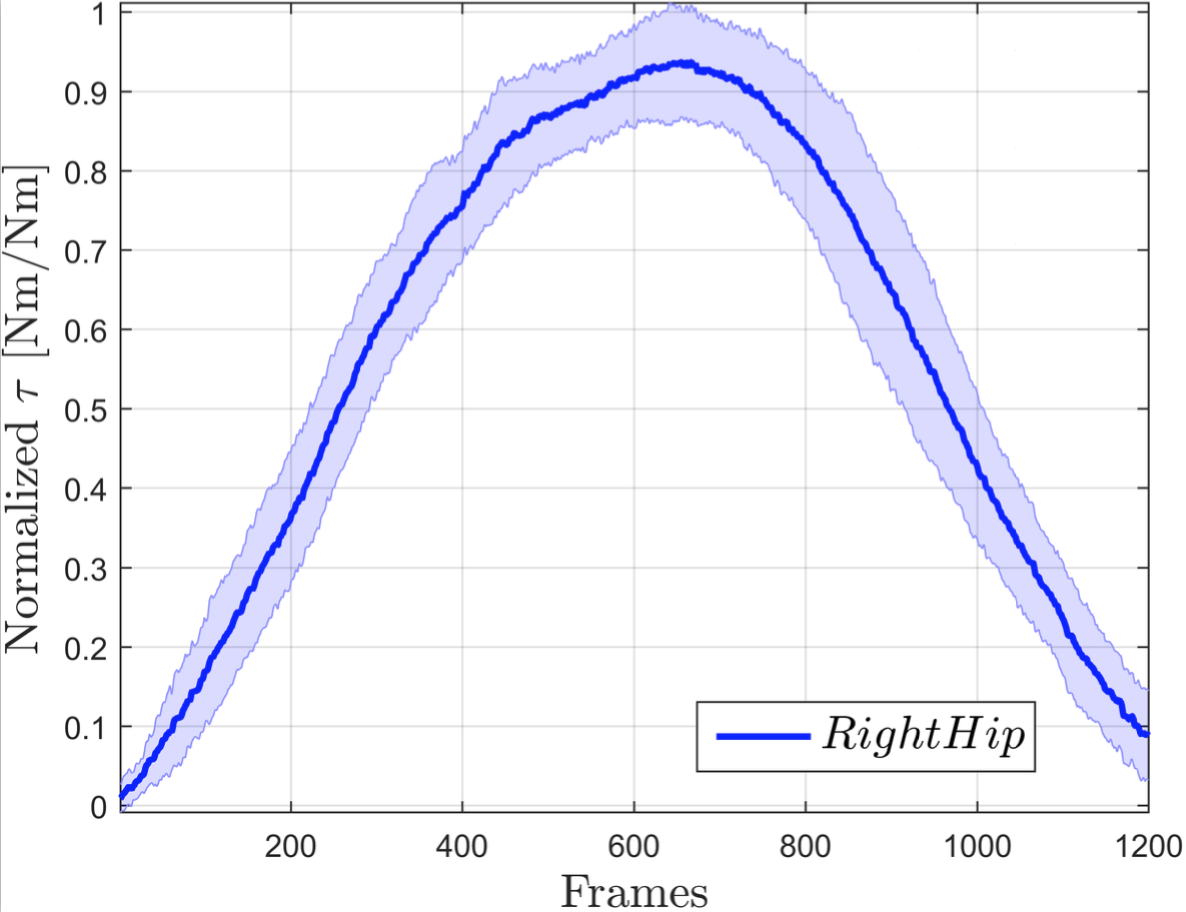
\includegraphics[width=0.48\textwidth]{figs/torqueRightHipBH}
	%	\caption{}
	%	\label{fig:figs_torqueRightHipBH}
	% \end{subfigure}
 %	\begin{subfigure}[b]{0.48\textwidth}
 		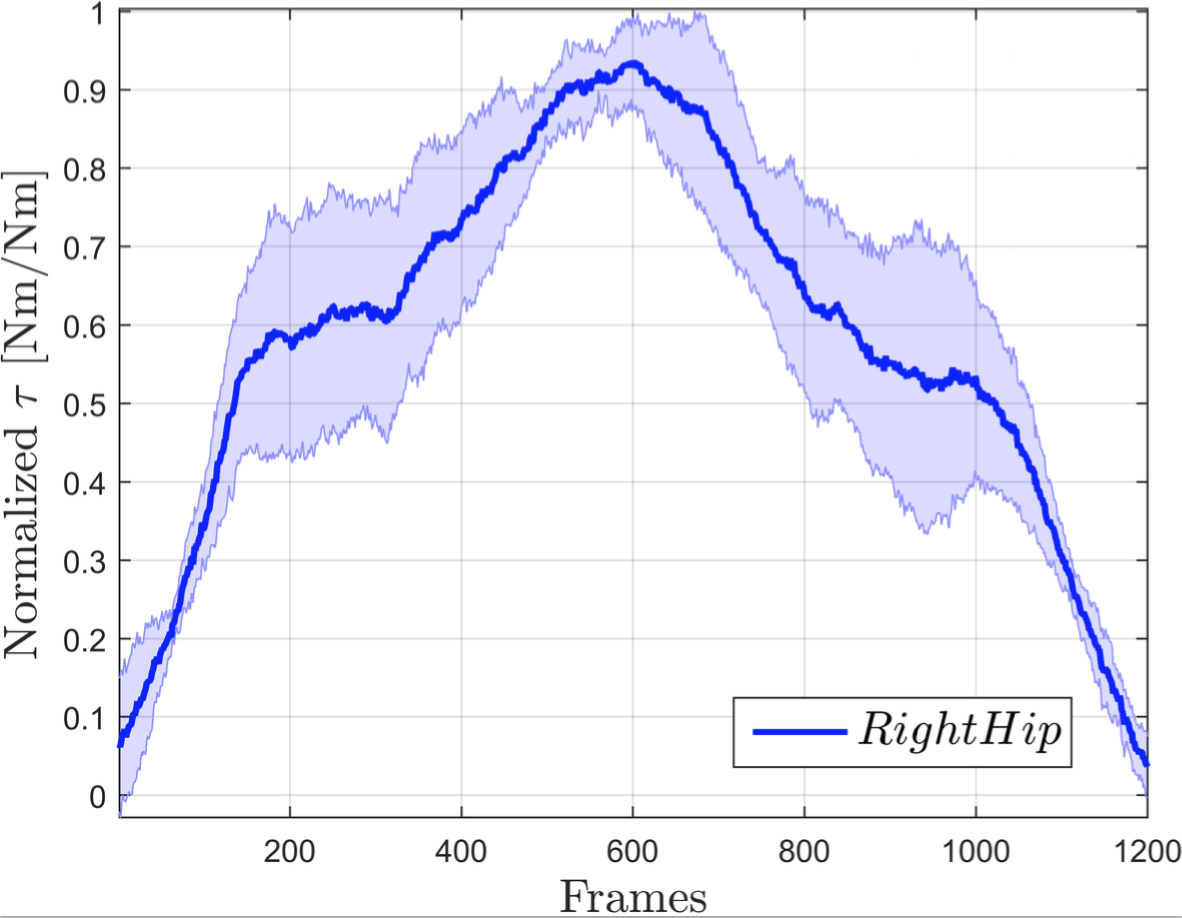
\includegraphics[width=0.48\textwidth]{figs/torqueRightHipBHR}
 %		\caption{}
 %		\label{fig:figs_torqueRightHipBRA}
 %	 \end{subfigure}
 %	\begin{subfigure}[b]{0.48\textwidth}                                                                 
   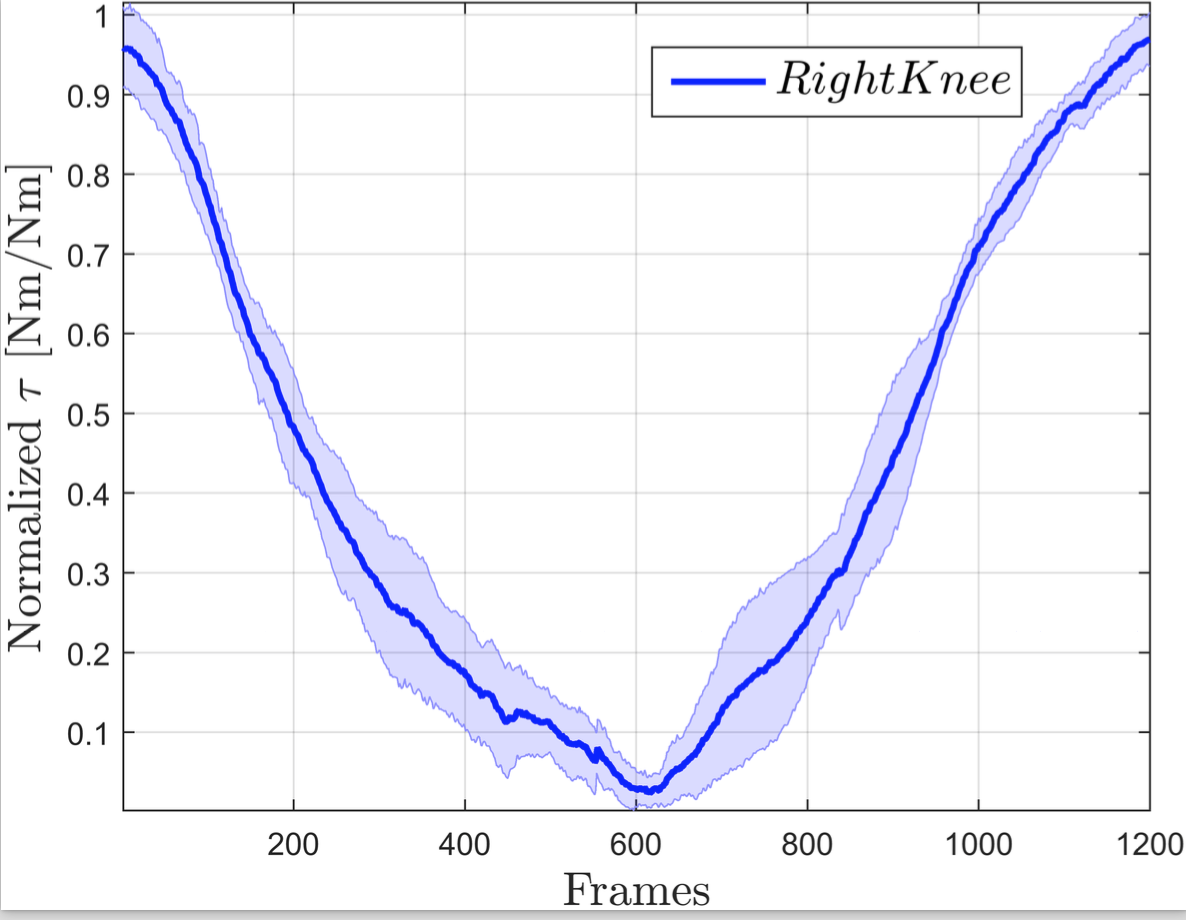
\includegraphics[width=0.48\textwidth]{figs/torqueRightKneeSH}
	%	 \caption{}
	%	\label{fig:figs_torqueRightKneeSH}
 %	 \end{subfigure}
 %	\begin{subfigure}[b]{0.48\textwidth}                                                         
 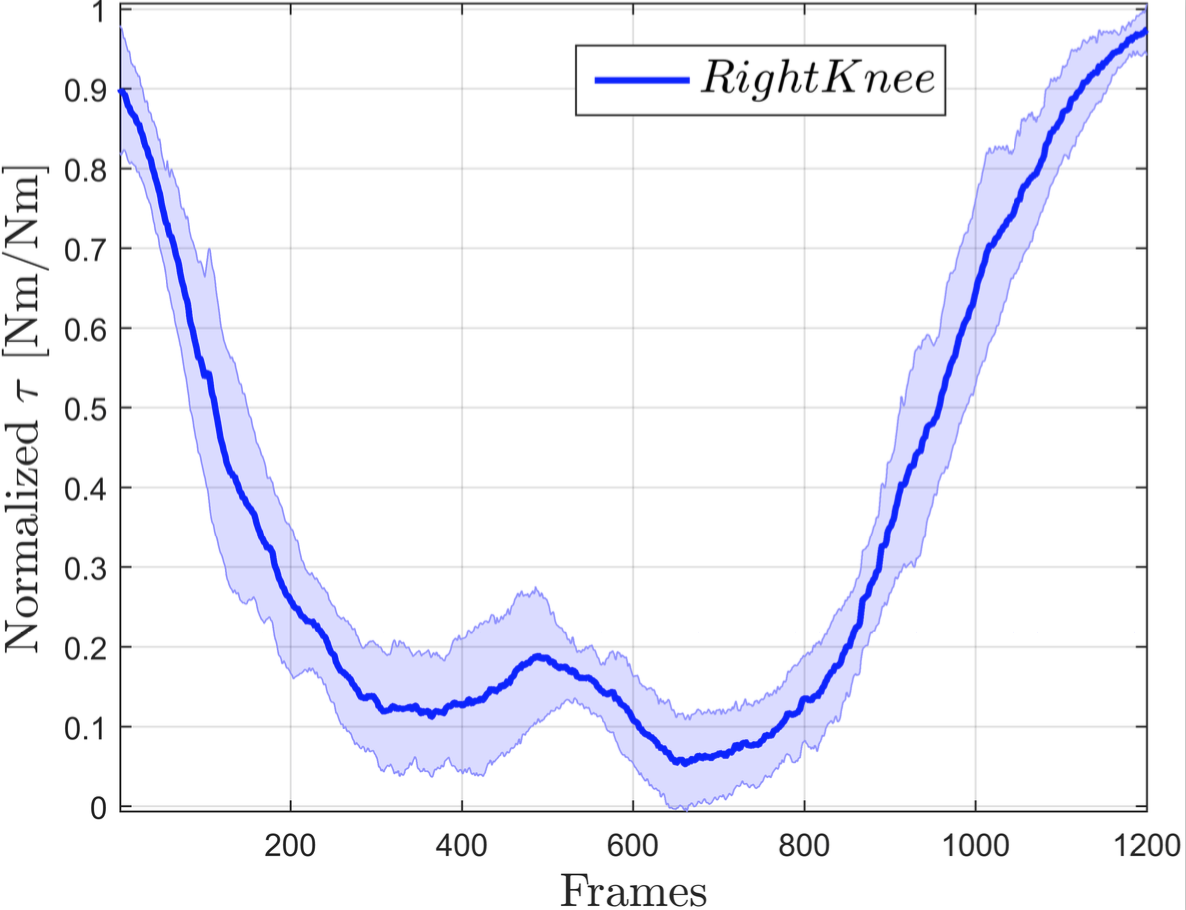
\includegraphics[width=0.48\textwidth]{figs/torqueRightKneeSHR}
 %		  	\caption{}
 	%	  	 \label{fig:figs_torqueRightKneeSR}
  %	 \end{subfigure}
      \caption{\emph{Inter-subjects analysis}: normalized torques of 10 subjects
		  (mean and standard deviation) for right hip in $BT$ without (a) and with (b) 
		  robot, for right knee in $ST$ without (c) and with (d) robot.}
 \end{figure*}
%
%%%%%%%%%%%%%%%%%%%%%%%%%%%%%%%%%%%%%%%%%%%%%%%%%%%%%%%%%%%%%%%%%%%%%%%%%%%%%%%%%%%%%%%%%%%%%%%%
\subsection{Robustness test}
To test the robustness of the method with respect to modeling errors we asked one subject to
perform the $BT$ with the robot in two different configurations, i.e. \emph{with} and
 \emph{without} an additional mass ($W$) of \unit{6}{\kilo}{\gram} roughly positioned in
  correspondence of the torso center of mass. The MAP computation was performed by
   considering as algorithm inputs the following cases (see Table \ref{table:robustness}):
	\begin{itemize}
		\item \emph{case A}: model of the subject without $W$ and measurements acquired 
		while performing the $BT$ with $W$;
		\item \emph{case B}: model of the subject without $W$ and measurements acquired 
		while performing the $BT$ without $W$.
		\end{itemize} 
Since in both the cases the analysis is performed with the model  of the subject without $W$, in
order to highlight a lower reliability for the model used in 
\emph{case A} computation, it is assigned a value to the model variance
\footnote{We refer here to the model covariance associated to the model as a diagonal matrix 
where each element of the diagonal is the variance value.}
 equal to $10^{-1}$ 
(different from the value of variance equal to $10^{-4}$ assigned for the \emph{case B}).
%
\begin{table}[H]
\caption{Cases for the MAP evaluation.}
\label{table:robustness}
\centering
\footnotesize
   \begin{tabular}{ l|| l | l | l | l | l | l | l | l  } 
    \multicolumn{1}{c||}{} &
    \multicolumn{3}{c|}{\emph{\textbf{case A}}} &
      \multicolumn{3}{c|}{\emph{\textbf{case B}}}\\
    \hline
	\hline
        \multicolumn{1}{|c||}{\emph{\textbf{model}}} &
    \multicolumn{3}{c|}{without W} &
      \multicolumn{3}{c|}{without W} \\
    \hline
    \multicolumn{1}{|c||}{\emph{\textbf{measurements}}} &
    \multicolumn{3}{c|}{with W} &
      \multicolumn{3}{c|}{without W}\\
	\hline
      \multicolumn{1}{|c||}{$\Sigma$ \emph{\textbf{model}}} &
      \multicolumn{3}{c|}{$10^{-1}$} &
        \multicolumn{3}{c|}{$10^{-4}$}\\
     \hline   
     % \hline
     \multicolumn{1}{|c||}{\emph{\textbf{MAP torque estimation}}} &
     \multicolumn{3}{c|}{$\bm \tau_{(model + \unit{6}{\kilo}{\gram})}$} &
       \multicolumn{3}{c|}{$\bm \tau_{model}$}\\
      \hline
    \end{tabular}
\end{table}
%
By exploiting the linearity property of the system we started by considering the 
following expression for the torques
\begin{eqnarray} \label{tauEq}
	\bm \tau_{(model + \unit{6}{\kilo}{\gram})} - \bm \tau_{model} = 
	\bm \tau_{\unit{6}{\kilo}{\gram}}
\end{eqnarray} 
where $\bm \tau_{\unit{6}{\kilo}{\gram}}$ is the theoretical torque due to the additional $W$
positioned on the torso\footnote{We consider a simple 2-DoF system (see \cite{LatellaSensors2016}) in which the position of $W$ and the hip joint angle are known.}.  Given \eqref{tauEq}, 
 it is possible to retrieve the error $\bm{\varepsilon}_{\bm{\tau}}$ on the $\bm \tau$ 
  estimation for the subject with $W$, due to \emph{case A}:
  %
\begin{eqnarray} \label{TorquesError}
	\bm{\varepsilon}_{\bm{\tau}} = |\bm \tau_{(model + \unit{6}{\kilo}{\gram})} -
	 \bm \tau_{model}| - \bm \tau_{\unit{6}{\kilo}{\gram}}
\end{eqnarray}
%
We computed \eqref{TorquesError} by using the OpenSim ID (Inverse Dynamics) toolbox 
as well, in order to evaluate its effectiveness with respect to the modeling errors.
Figures \ref{fig:MAPtau_cmp}-\ref{fig:OPENSIMtau_cmp} provide the mean and the standard deviation of the torque estimation by means of the MAP algorithm and the OpenSim software, respectively.  Figure \ref{fig:BOXPLOT} shows the comparison between the computation of the error in \eqref{TorquesError} for both the above methods: the error is higher in OpenSim computation than in MAP since OpenSim does not offer the possibility of setting the model reliability in the computation.
%
% \begin{figure}[h!]
%   \centering
%    \begin{subfigure}[b]{1\columnwidth}
%       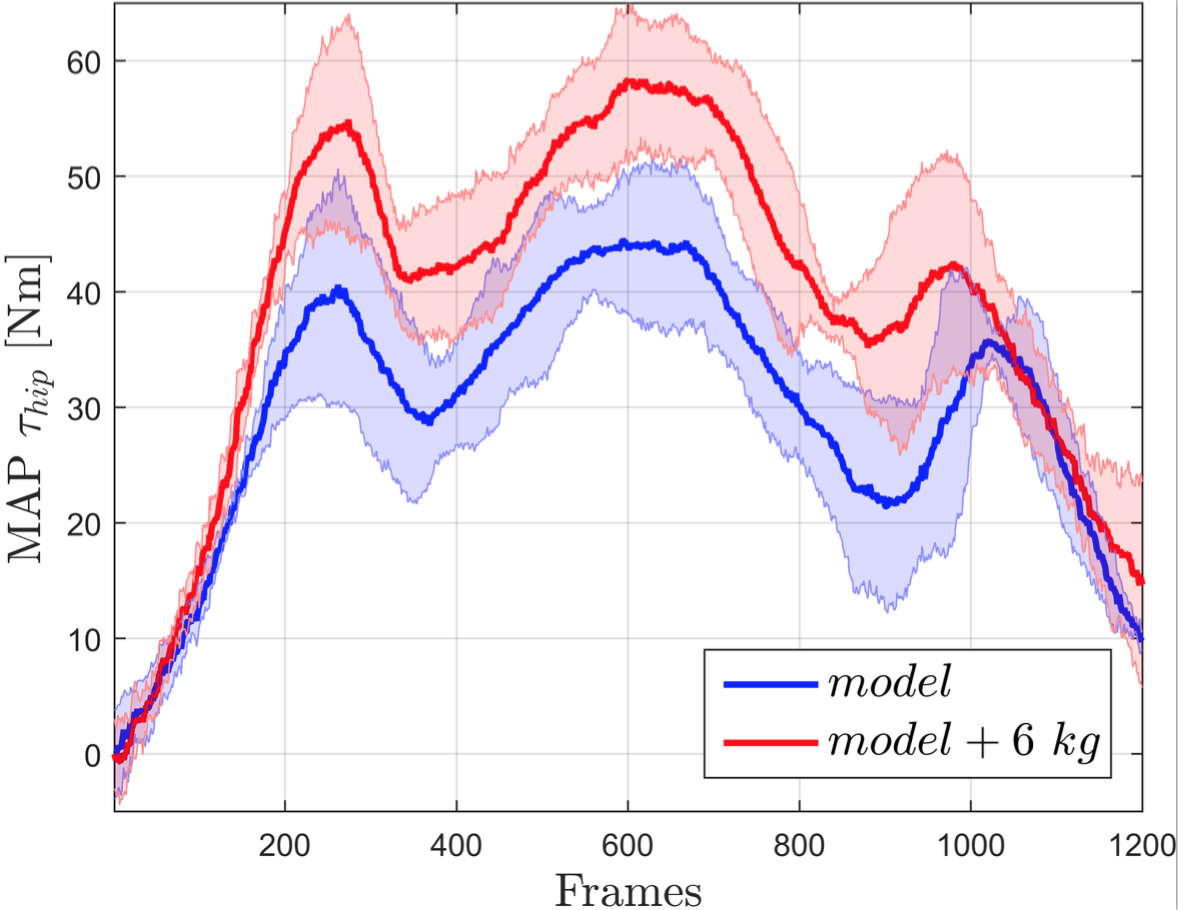
\includegraphics[width=\textwidth]{figs/TorqueComparison.pdf}
%           \caption{}
%           \label{fig:figs_torqueRightHipBH}
%   \end{subfigure}
%    \begin{subfigure}[b]{1\columnwidth}
%     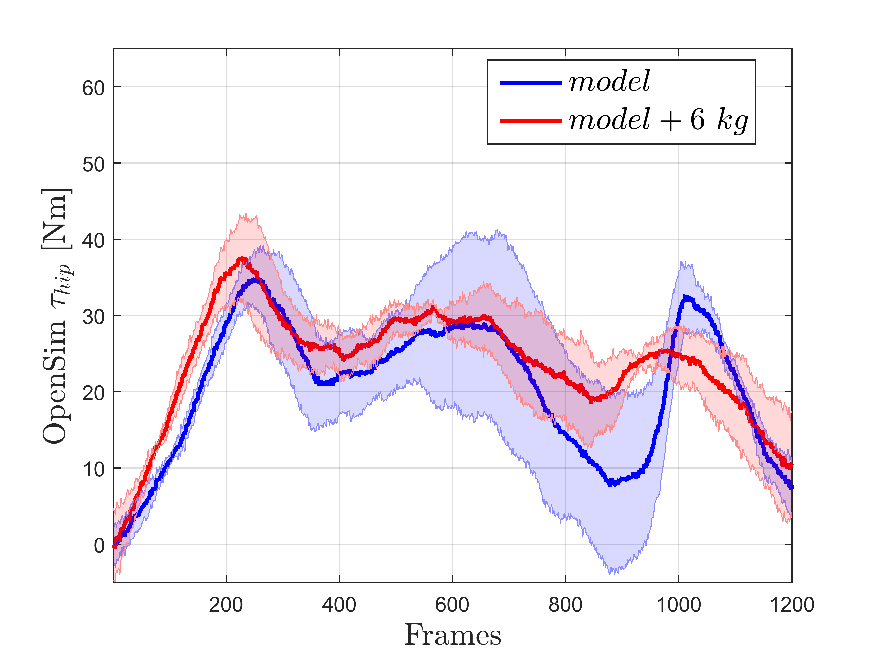
\includegraphics[width=\textwidth]{figs/TorqueComparisonOPENSIM.pdf}
% 	\caption{}
%         \label{fig:figs_torqueRightKneeSR}
%    \end{subfigure}
%           \caption{\emph{Intra-subjects analysis}: }
% \end{figure}
%
 \begin{figure*}[!ht]
	 \centering
%	\begin{subfigure}[b]{0.33\textwidth}
		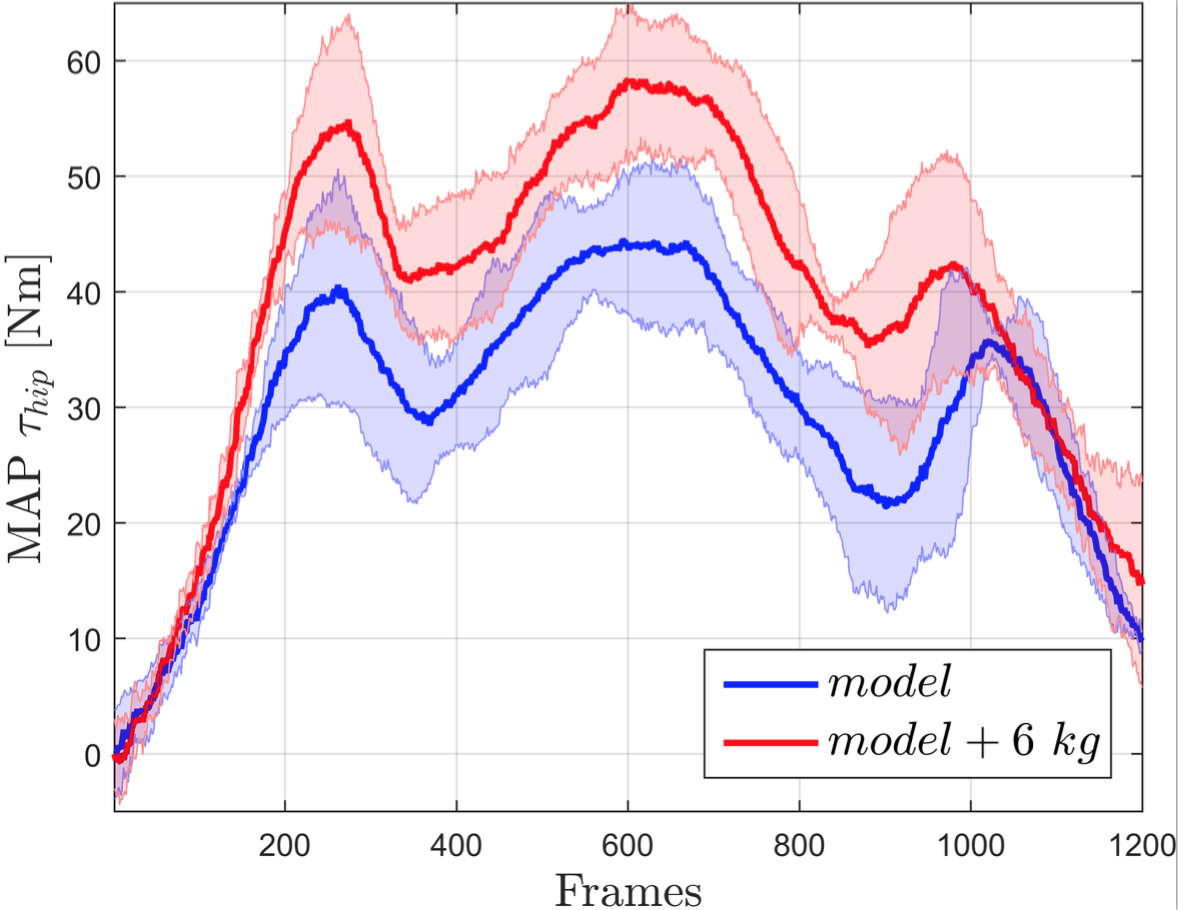
\includegraphics[width=0.3\textwidth]{figs/TorqueComparison}
%		\caption{}
%		\label{fig:MAPtau_cmp}
%	 \end{subfigure}
% 	\begin{subfigure}[b]{0.33\textwidth}
 		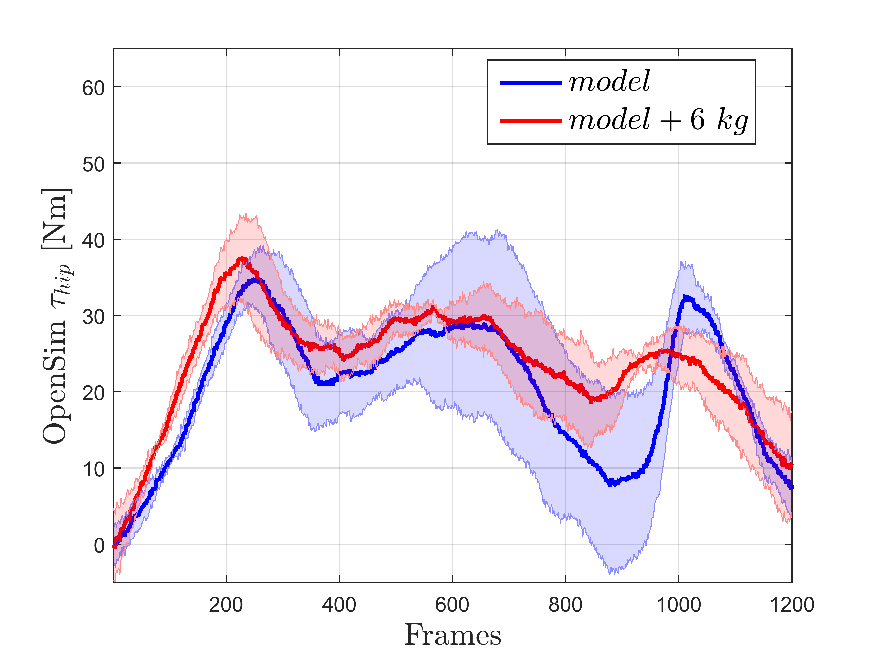
\includegraphics[width=0.3\textwidth]{figs/TorqueComparisonOPENSIM.pdf}
% 		\caption{}
%		\label{fig:OPENSIMtau_cmp}
% 	 \end{subfigure}
%  	\begin{subfigure}[b]{}
  		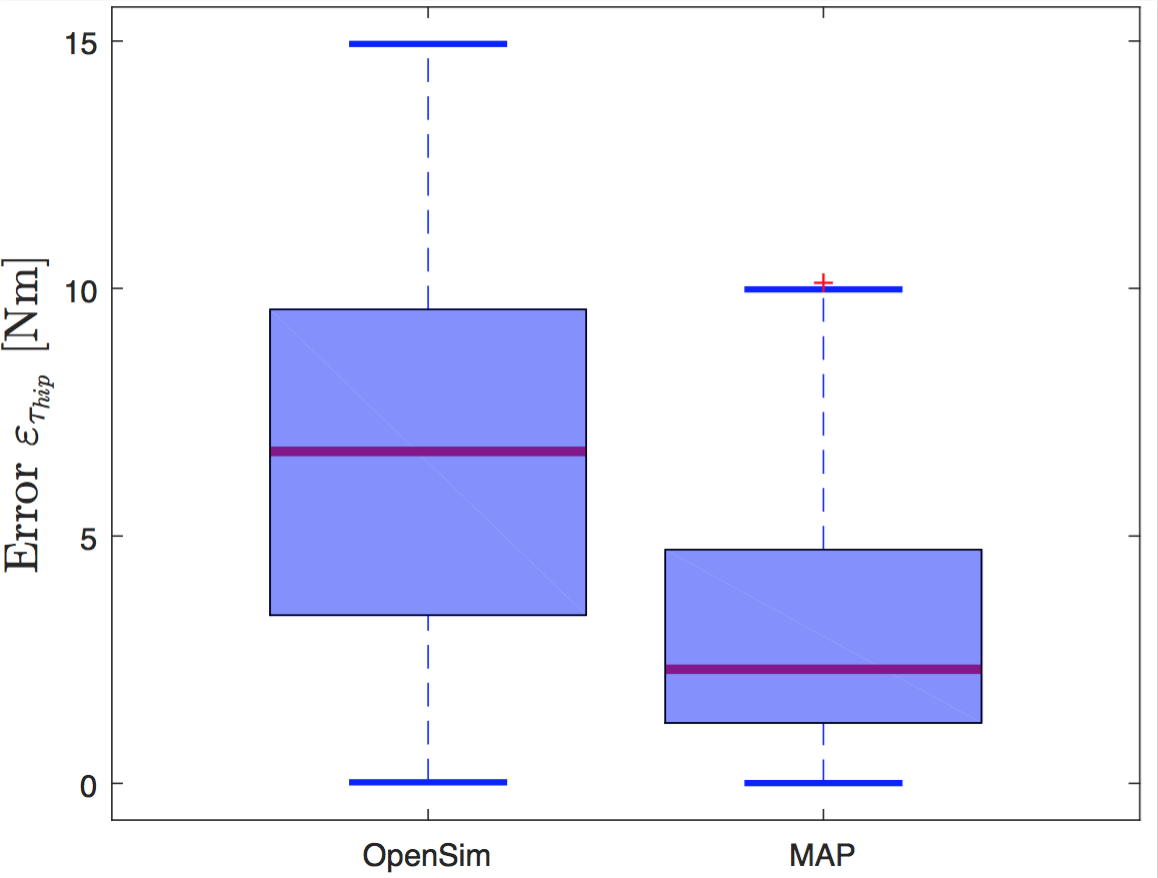
\includegraphics[width=0.3\textwidth]{figs/OPENSIMvsMAP}
%  		\caption{}
%		\label{fig:BOXPLOT}
%  	 \end{subfigure}
     \caption{\emph{Intra-subjects analysis}: mean and standard deviation of $\bm \tau$
	  (i.e., the sum of the $\bm \tau$ estimated at the hips)
	 among five repetitions of the $BT$ performed by a subject computed for \emph{case A} 
	 (red) and \emph{case B} (blue) by means of (a) MAP algorithm  and (b) by using the 
	 OpenSim ID (Inverse Dynamics) toolbox. (c) Box plots of the torque estimation error
	 $\bm{\varepsilon}_{\bm{\tau}}$ computed in \eqref{TorquesError} with MAP (on the right)
	 and with OpenSim (on the left). It shows that MAP is a method more robust to the
	 modelling errors since it gaves the possibility of weighting the reliability of the model
	  by properly setting the related covariance matrix. }
 \end{figure*}

%%%%%%%%%%%%%%%%%%%%%%%%%%%%%%%%%%%%%%%%%%%%%%%%%%%%%%%%%%%%%%%%%%%%%%%%%%%%%%%%%%%%%%%%%%%%%%%%
\subsection{Incremental sensor fusion analysis}
Since a distinctive feature of our framework consists in the possibility of building
 \eqref{eq:measRNEA} for different sources of measurement, we here investigate the advantage in
  using this algorithm for the dynamics estimation. We consider three sets of $\bm y$ 
  equations for: 
\begin{enumerate}
	\item  the two force plates: 
	\begin{eqnarray}
		\bm{y}_{\mbox{\scriptsize{\emph{FP}}}} & = & {}^{{\mbox{\scriptsize{\emph{FP}}}}}
		\bm{X}_{\mbox{\scriptsize{\emph{hFOOT}}}}~\bm{f}_{\mbox{\scriptsize{\emph{hFOOT}}}}
	\end{eqnarray}
	where it is used the trasformation matrix\footnote{See \cite{Featherstone2008}
	 for the definition of the trasformation
	 matrix between two reference frames.} $\bm X$  between the human foot reference frame 
	(${\mbox{\footnotesize{\emph{hFOOT}}}}$) and each force plate frame
	 (${\mbox{\footnotesize{\emph{FP}}}}$);
	\item  the IMUs embedded in the suit:
	\begin{eqnarray}
		\bm{y}_{\mbox{\scriptsize{\emph{IMU}}}} & = &
		 {}^{\mbox{\scriptsize{\emph{IMU}}}}\bm{X}_{\mbox{\scriptsize{\emph{L}}}}~
		 \bm{a}_{\mbox{\scriptsize{\emph{L}}}}
	\end{eqnarray}
	by exploiting the trasformation between each human link frame
	 ${\mbox{\footnotesize{\emph{L}}}}$ 
	on which the IMU is attached and
	that particular IMU reference frame (Fig. \ref{fig:figs_human_JointLink}a);  
	\item  the force/torque sensors of the two arms of the robot:
	\begin{eqnarray}
		\bm{y}_{\mbox{\scriptsize{\emph{iCubFT}}}} & = &
		 {}^{\mbox{\scriptsize{\emph{iCubFT}}}}\bm{X}_{\mbox{\scriptsize{\emph{hHAND}}}}~
		 \bm{f}_{\mbox{\scriptsize{\emph{hHAND}}}}
	\end{eqnarray}
	for which it is necessary knowing the transformation between each human hand frame
	(${\mbox{\footnotesize{\emph{hHAND}}}}$)
	to the robot sensor frame (${\mbox{\footnotesize{\emph{iCubFT}}}}$).
\end{enumerate}

\indent
A general overview of the above-mentioned frames is shown in Fig.
 \ref{fig:interaction_lateral&top}a. We want to prove that, by adding progressively 
 the different sensors data at each MAP computation, the variance associated to 
 the estimated dynamic variables consequently decreases, making the estimation more reliable.
%
In particular, we build \eqref{eq:measRNEA} for three different cases (Fig.
 \ref{fig:sensAddition&barAnalysis}a) :
\begin{itemize}
\item[\textit{case 1)}]  $\bm{y} = [\bm{\ddot{q}},~\bm{y}_{\mbox{\scriptsize{\emph{FP}}}}]$
\item[\textit{case 2)}] $\bm{y} = [\bm{\ddot{q}},~\bm{y}_{\mbox{\scriptsize{\emph{FP}}}},~ \bm{y}_{\mbox{\scriptsize{\emph{IMUs}}}}]$ 
\item[\textit{case 3)}] $\bm{y} = [\bm{\ddot{q}},~\bm{y}_{\mbox{\scriptsize{\emph{FP}}}},~ \bm{y}_{\mbox{\scriptsize{\emph{IMUs}}}},~\bm{y}_{\mbox{\scriptsize{\emph{iCubFT}}}}]$.
\end{itemize}
%
The MAP computation is performed for each case since the incremental addition of a sensor 
includes each time a new information on the analysis.  
For this analysis we take into account a task involving the robot ($BT$) in order to 
include the robot sensor measurements in the computation.  Among the variables in $\bm d$ we consider again the torque $\bm \tau$ (i.e., right and left ankle and hip) and the variance along the axis of major relevance $y$.

 \begin{figure*}[!ht]
	 \centering
		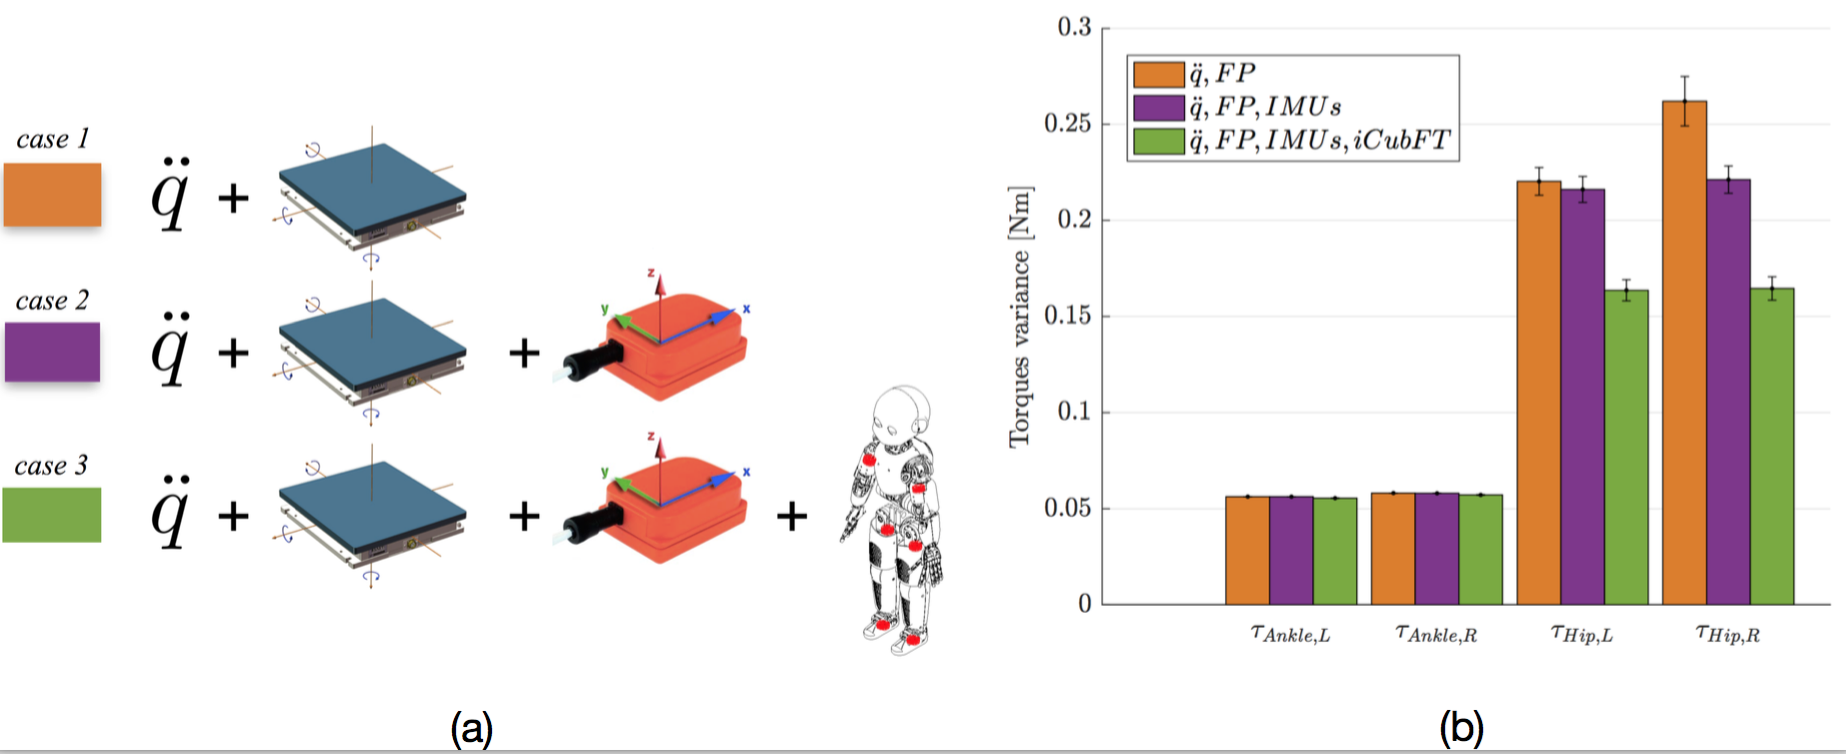
\includegraphics[width=0.9\textwidth]{figs/sensAdditionAndBarAnalysis}
      \caption{(a) Description of three cases for progressive addition of sensors.
	   (b) \emph{Inter-subjects analysis}: mean variance of $\bm \tau$ at the left and right
	    ankle and hip among five repetitions of the $BT$ performed by ten subjects computed 
		by MAP with the three different version of the measurements vector $\bm y$.}
		 		\label{fig:sensAddition&barAnalysis}
 \end{figure*}
% 
 % \begin{figure*}[h!]
 % 	 \centering
 % 	\begin{subfigure}[b]{0.48\textwidth}
 % 		\includegraphics[width=\textwidth]{figs/sensAddition.pdf}
 % 		\caption{}
 % 		\label{fig:figs_sensAdd}
 % 	 \end{subfigure}
 % 	\begin{subfigure}[b]{0.48\textwidth}
 % 		\includegraphics[width=\textwidth]{figs/SDall.pdf}
 % 		\caption{}
 % 		\label{fig:figs_SDall}
 % 	 \end{subfigure}
 %      \caption{(a) Description of three cases for progressive addition of sensors.
 % 	   (b) \emph{Inter-subjects analysis}: mean variance of $\bm \tau$ at the left and right
 % 	    ankle and hip among five repetitions of the $BT$ performed by ten subjects computed
 % 		by MAP with the three different version of the measurement vector $\bm y$.}
 % \end{figure*}
 %
Passing progressively from \textit{case 1} to \textit{case 3} (Fig. \ref{fig:sensAddition&barAnalysis}a)
the variance associated to the torques decreases\footnote{In order to assess 
the statistical significance of results, a paired-samples
 \emph{t-test} is performed firstly between \textit{case 1} and \textit{case 2} 
 ($2$ sensors vs $3$ sensors) and then between \textit{case 2} and \textit{case 3} 
 ($3$ sensors vs all sensors).  Torque variances statistically significant,  
  \emph{p-value} $<0.05$.}. In Fig. \ref{fig:sensAddition&barAnalysis}b we show 
the decreasing behaviour of the mean variance of the torque at the hips and at the ankles
 computed between ten subjects.
%
The variance values on the ankles do not change significantly among the three different
 configurations of sensors since the ankle torque estimation depends mostly on the 
 contribution of the force plates that are included in all the three 
 cases of the computation.  Conversely, a significant decreasing behaviour is present 
 in the values associated to the hips. In this case the contribution of the three sources 
 of sensors becomes important since the torque estimation at the hips are affected 
 by the all sensors.